\section{Coche}

La composición del coche es muy similar al usado en la práctica 2, con la misma jerarquía, pero los cilindros de las ruedas tienen menos aristas, para acentuar el efecto de movimiento de las ruedas. Además, como se pide que la espada deba mirar a la parte superior del vehículo, he usado un \textit{Dummy} para que mire correctamente. Si bien se podría haber hecho con el cubo de arriba, me ha parecido más correcto hacer esto, ya que no va a mirar al centro del coche, sino a la parte trasera.

\bigskip

Voy a dividir cada restricción, incluyendo la de la espada, en subsecciones:


% ACTUALIZAR ESTA SECCION SI SE CAMBIA EL LUNES ALGO
% QUIZAS RESCRIBIR ALGUNAS FRASES, QUE SON RARAS
\subsection{Configuración de la espada para que gire}

Para que la espada mire, es necesario utilizar la restricción \textit{LookAt Constraint}, junto al \textit{Select LookAt Axis} en el eje Z, para que funcione correctamente. Con esto hecho, hace falta seleccionar los \textit{Targets}, que en mi caso son dos:

\begin{itemize}
    \item Un primer \textit{Dummy} que siempre se encuentra encima de la espada para que esta apunte hacia arriba en un primer momento. Este objeto tiene una restricción \textit{Link}, que está unida a las manos y la plataforma, haciendo que así siga siempre a la espada.
    
    Además, he bloqueado la herencia de rotación y escalado, para que sea muy similar al \textit{Position Constraint}, pero más flexible en términos de ajustar el \textit{dummy} a la escena.

    Esto se puede hacer yendo a \textit{Hierarchy} $\rightarrow$ \textit{Link Info}:

    \begin{figure}[H]
        \centering
       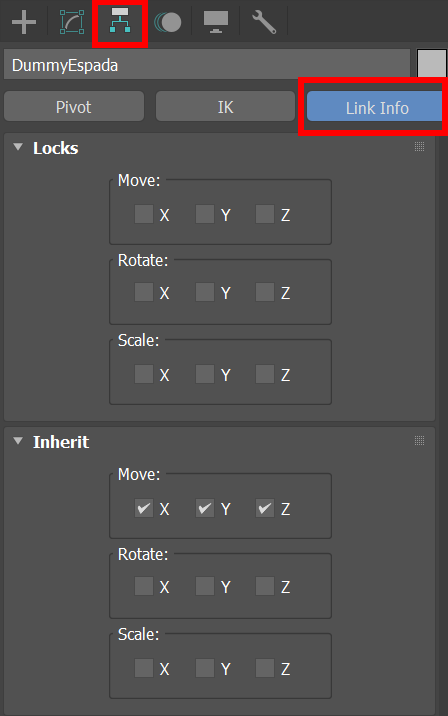
\includegraphics[width=0.35\textwidth]{imagenes/espada/dummyTopHierarchy.png}
       \caption{Menú para bloquear canales.}
    \end{figure}

    \item El segundo \textit{Dummy} es el comentado anteriormente, uno que se encuentra en la parte trasera superior del coche.
\end{itemize}

Con esto hecho, solo falta hacer una transición suave de un \textit{target} a otro. Entonces, los instantes referentes a esta restricción son:

\begin{itemize}
    \item \textbf{Instante 125: }La espada sigue mirando al \textit{dummy} que tiene justo encima.
    \item \textbf{Instante 150: }La espada ahora está mirando completamente hacia el \textit{dummy} del coche.
\end{itemize}

Las curvas de animación de la restricción son:

% curvas de la restricción
\begin{figure}[H]
    \centering
   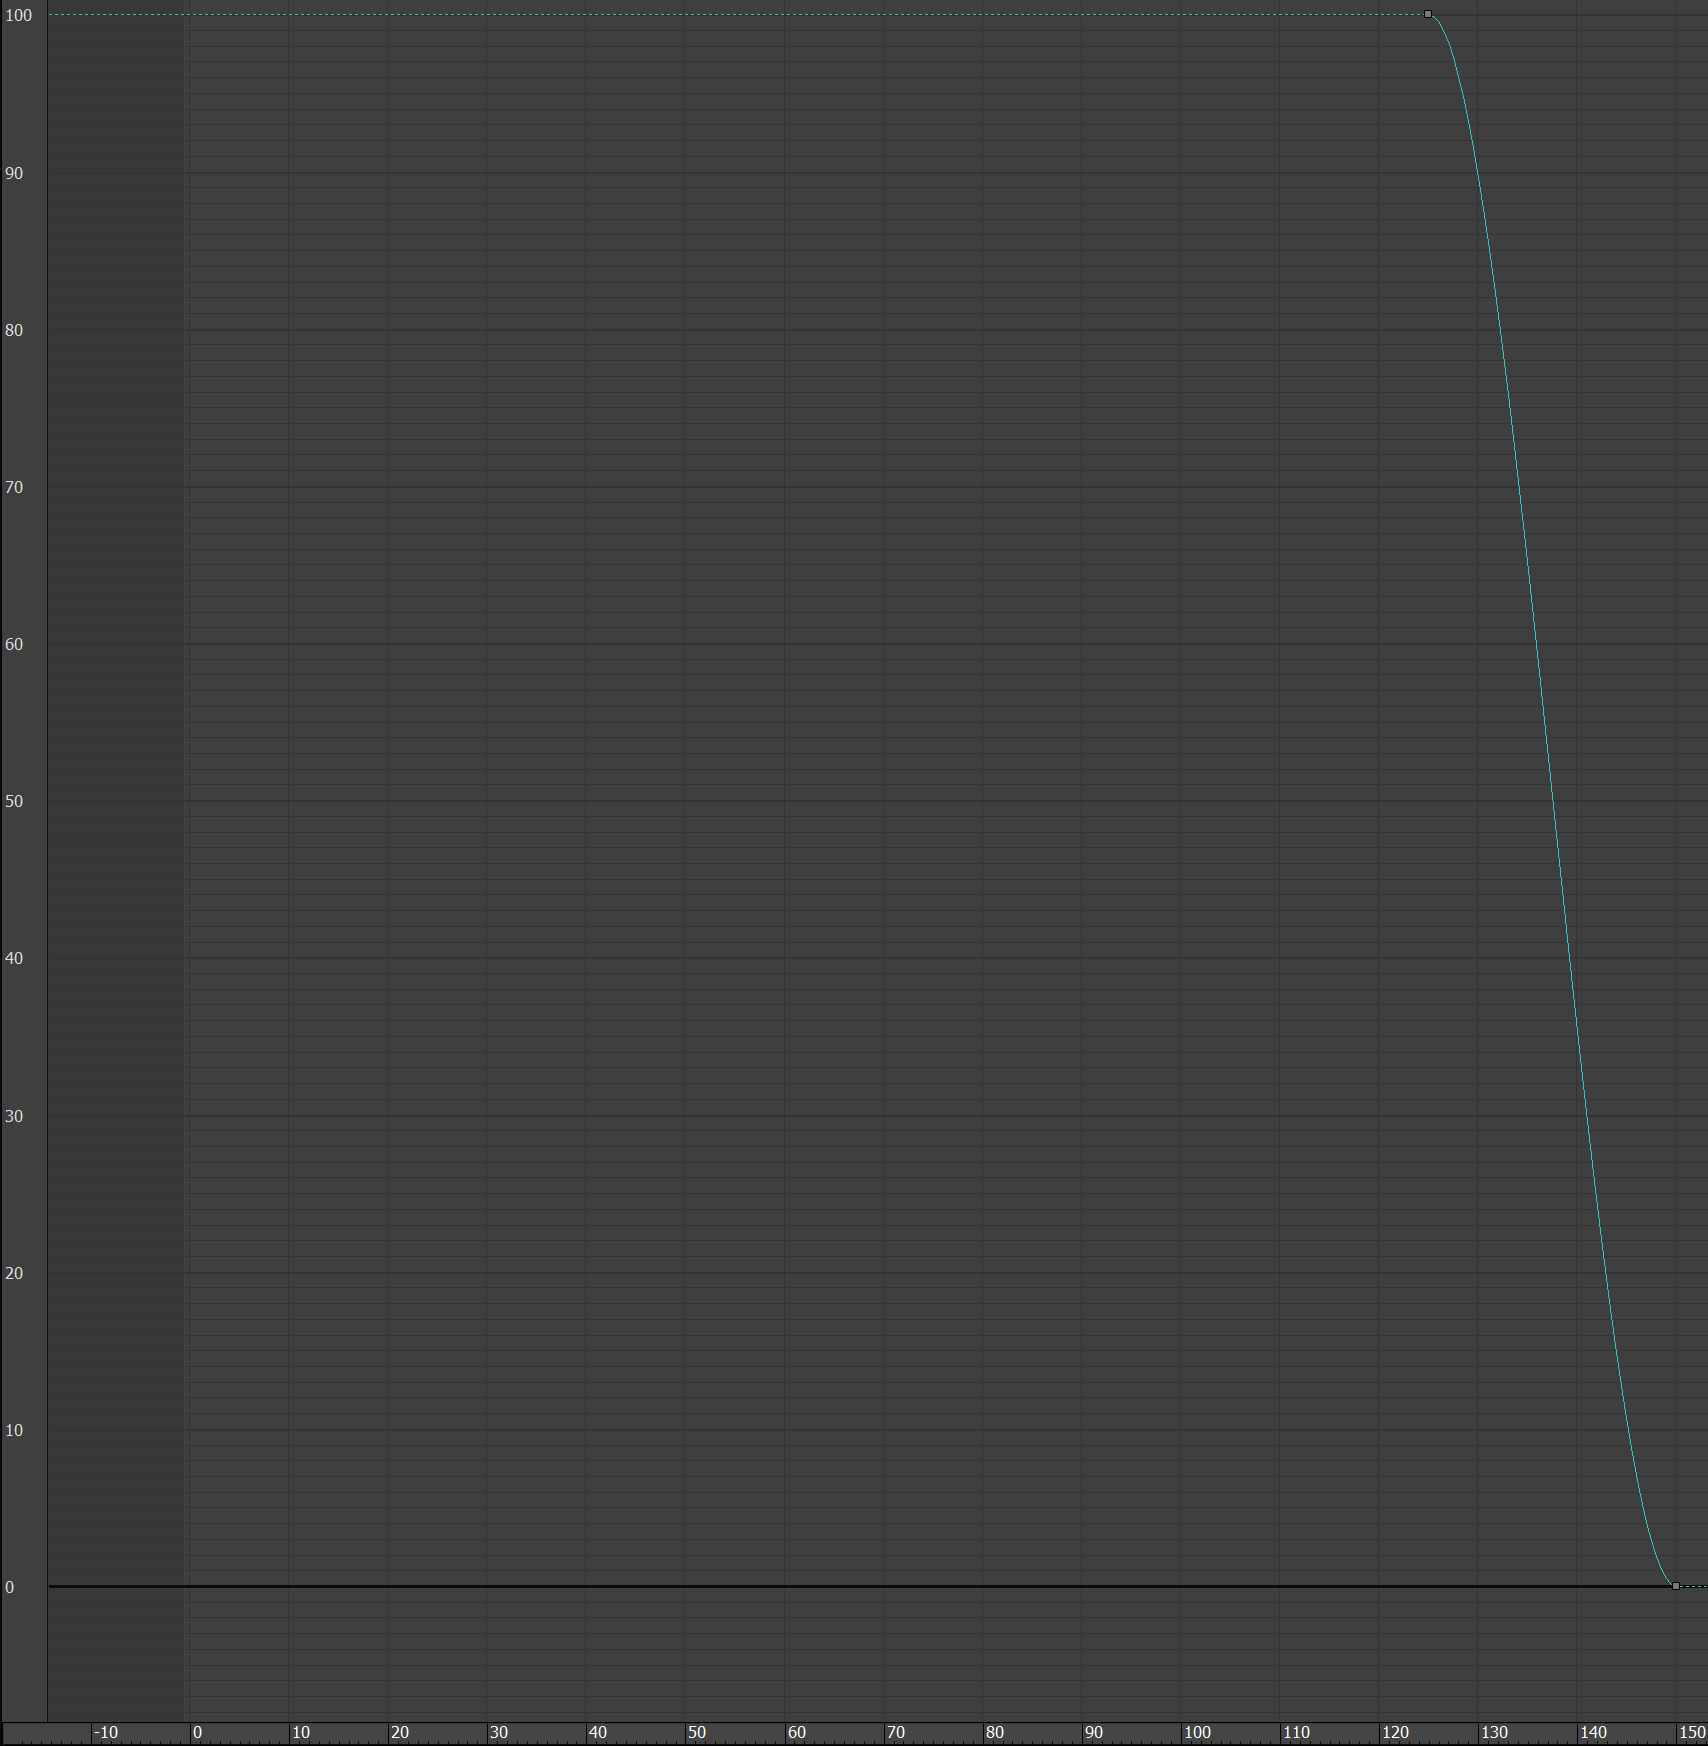
\includegraphics[width=0.6\textwidth]{imagenes/espada/lookat0.png}
   \caption{Curva usada para realizar el cambio de pesos en la restricción en el objetivo del \textit{dummy}.}
\end{figure}

\begin{figure}[H]
    \centering
   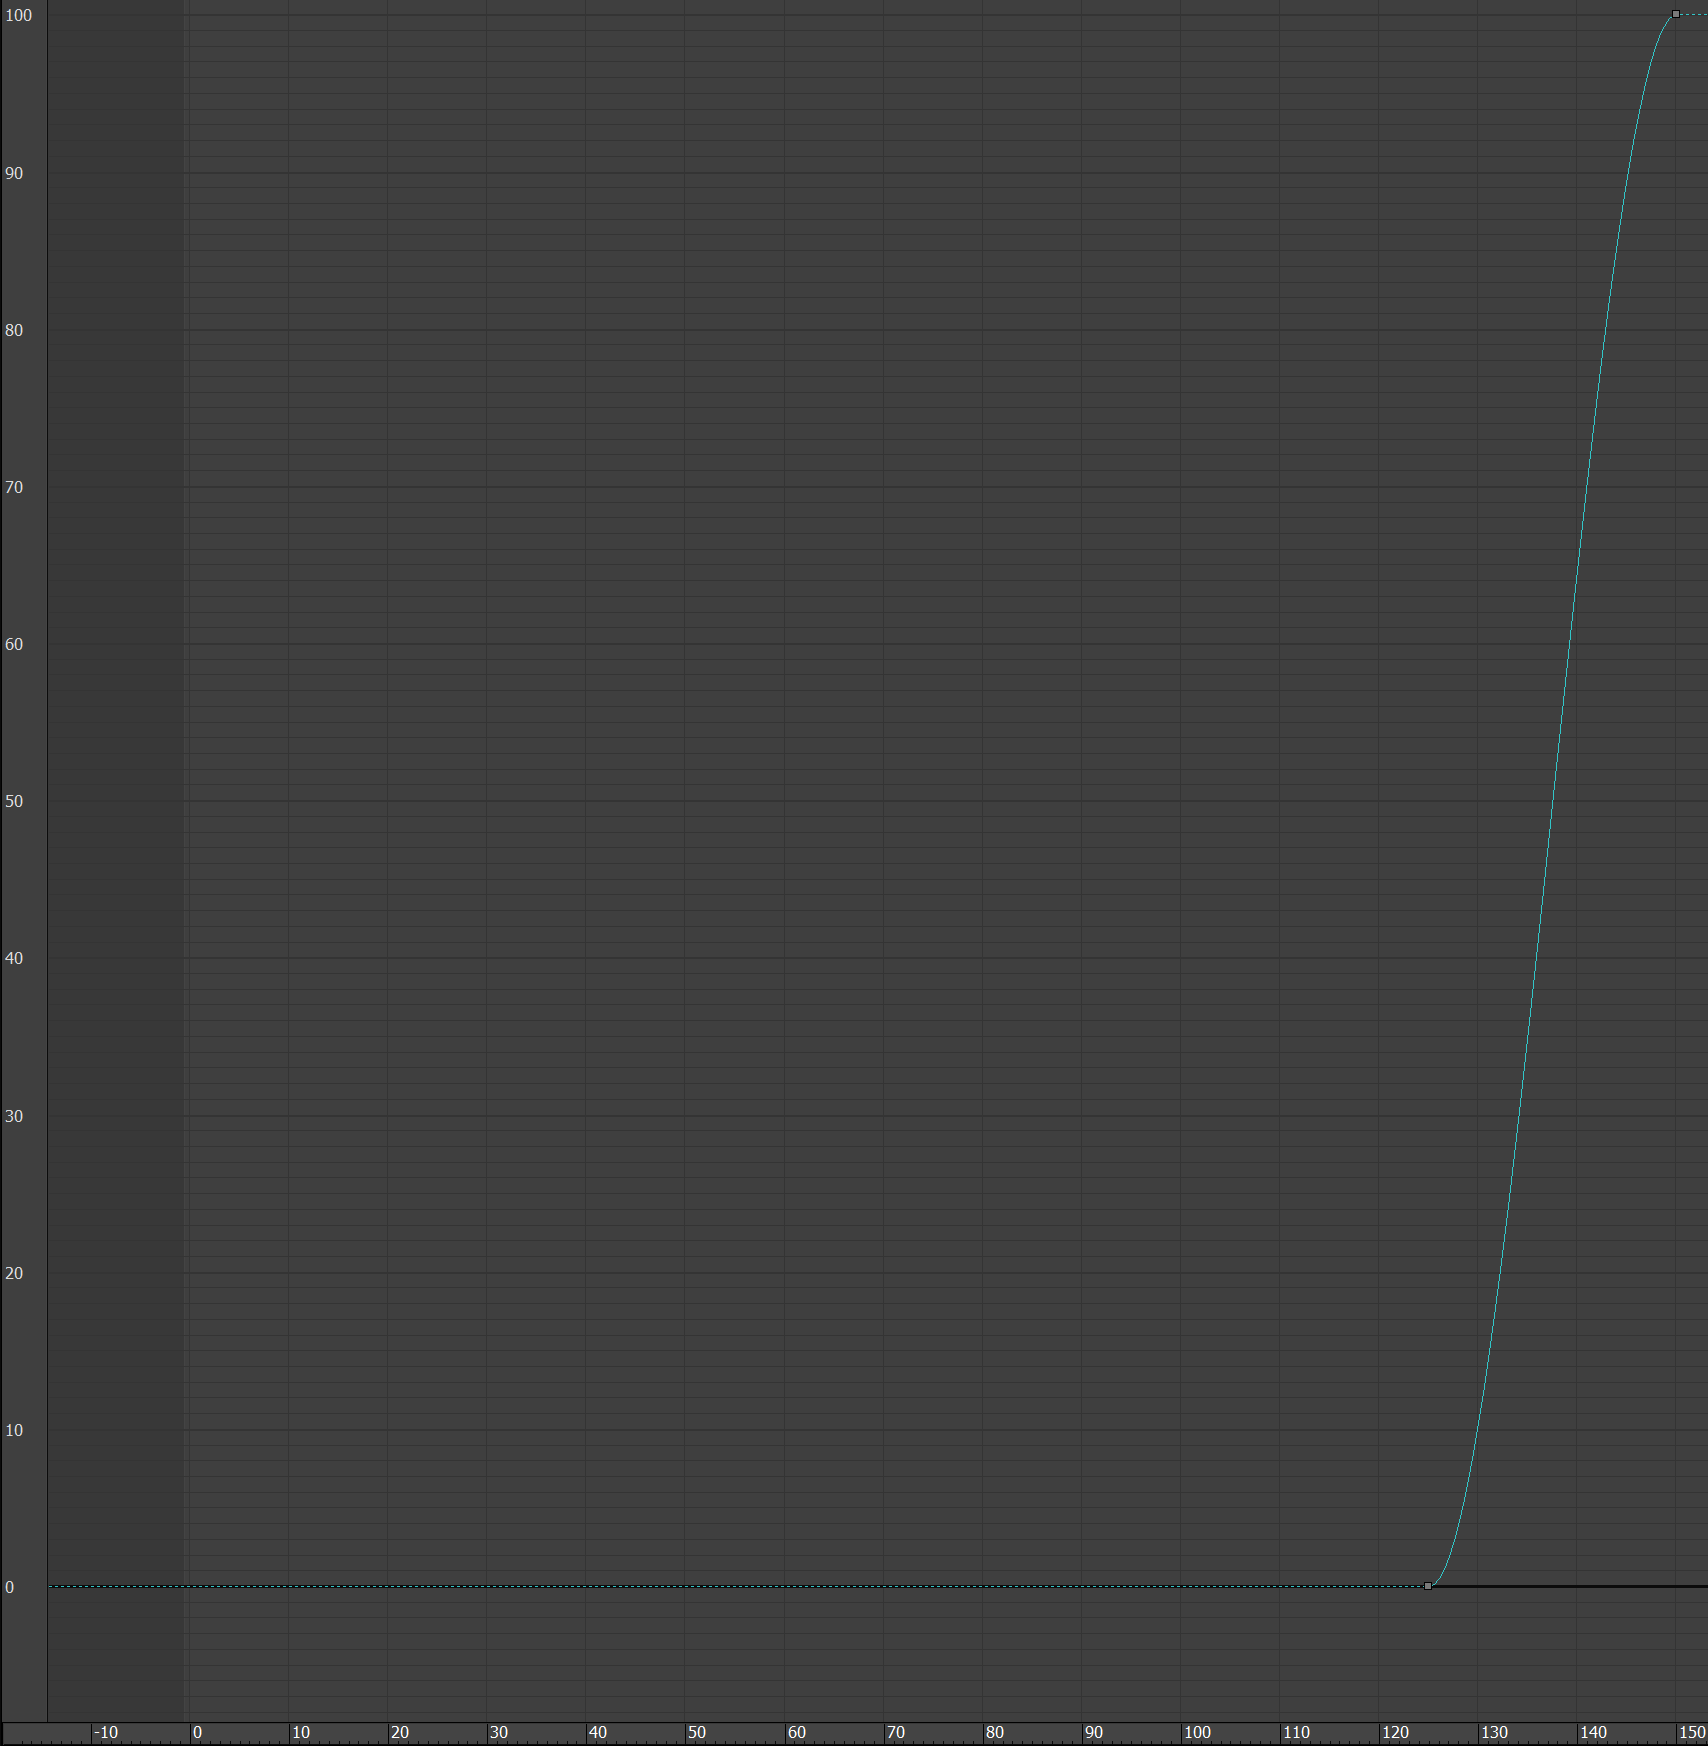
\includegraphics[width=0.6\textwidth]{imagenes/espada/lookat1.png}
   \caption{Curva usada para realizar el cambio de pesos en la restricción en el objetivo del \textit{dummy} del coche.}
\end{figure}

Como se puede ver, he utilizado la forma de la curva \textit{Slow-in/Slow-out}, ya que probando otros tipos no me han parecido del todo realistas.

\bigskip

Además, la configuración final del \textit{LookAt Constraint} es:

\begin{figure}[H]
    \centering
   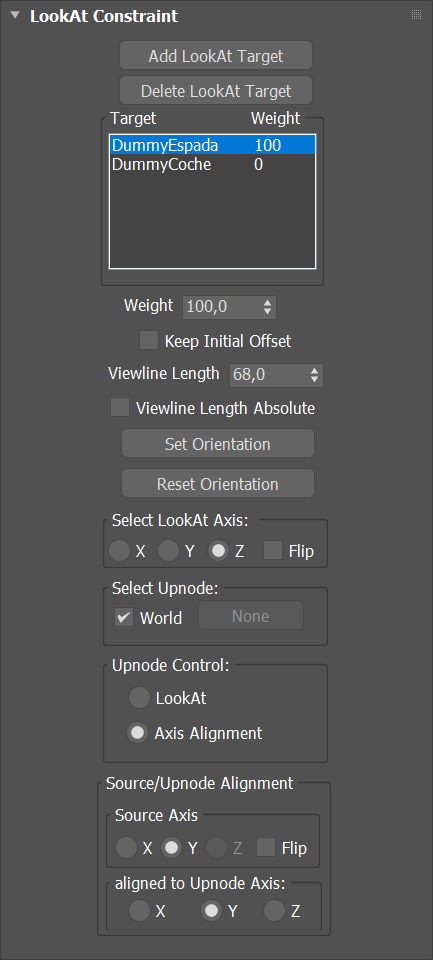
\includegraphics[width=0.3\textwidth]{imagenes/espada/lookatconfig.png}
   \caption{Configuración final del \textit{LookAt Constraint} en el espada.}
\end{figure}

% rescribir esta parte, digo mucho en mi caso
\subsection{Seguimiento de la curva}

Lo primero que hay que hacer es generar un spline que será usado por el coche para realizar la ruta.

\begin{figure}[H]
    \centering
   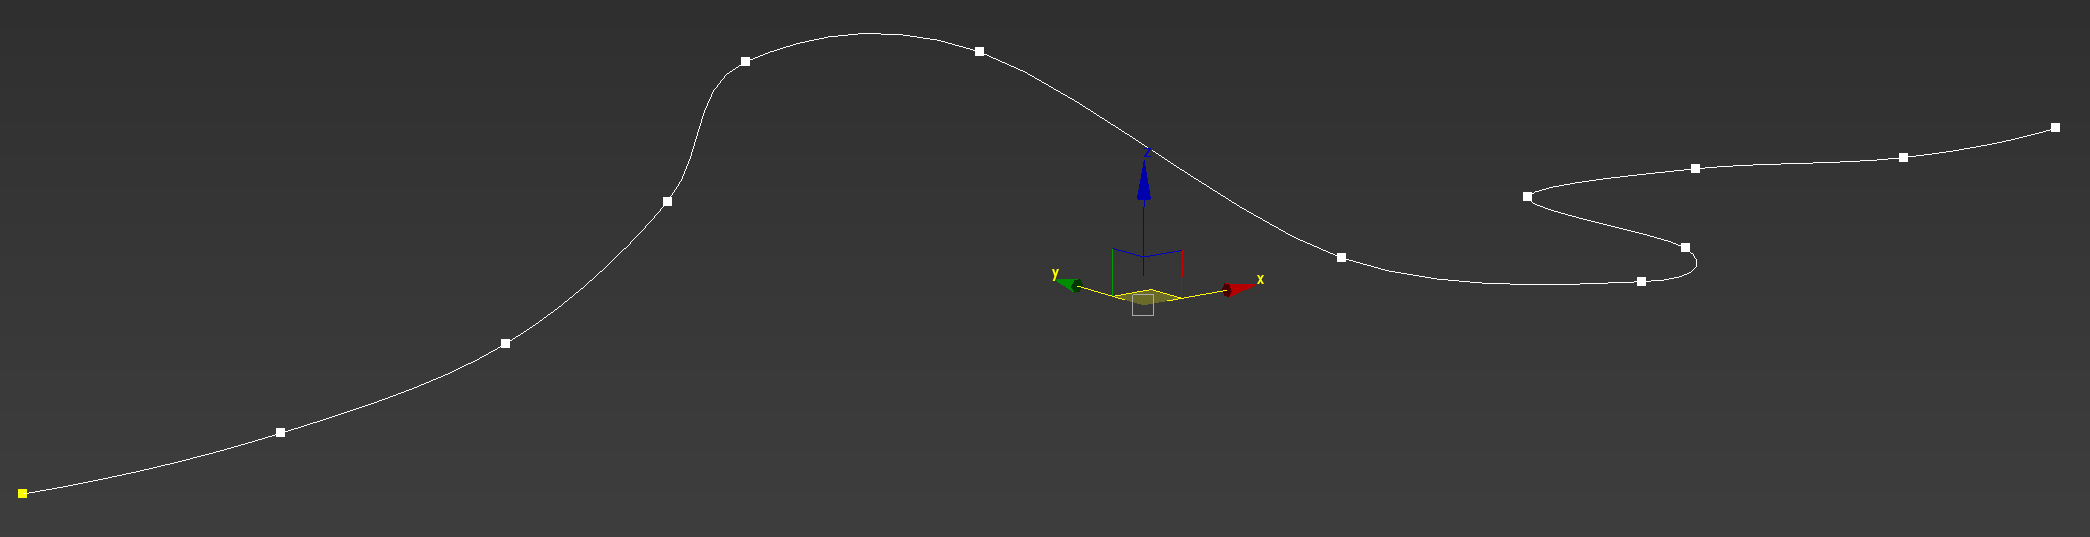
\includegraphics[width=0.6\textwidth]{imagenes/spline/spline.png}
   \caption{Forma que tiene el spline, se puede ver que sube y baja también.}
\end{figure}

Una vez generado, es necesario ponerle al coche la restricción \textit{Path Constraint} con el \textit{Path} creado anteriormente. En mi caso he decidido ponérselo al padre de la jerarquía, que es el cubo inferior. Además, hay que habilitar la opción \textit{Follow} para que el coche lo siga y deshabilitar la opción \textit{Loop} para que no siga infinitamente.

\bigskip

Una vez hecho esto, simplemente es necesario modificar los \textit{keyframes} de inicio y final para que vaya más lento, que en mi caso han sido los instantes \textbf{150} y \textbf{300}.

\bigskip

Tras hacer esto, se puede ver como el coche se mueve siguiendo el spline de manera correcta.

\bigskip

La curva de animación es:

\begin{figure}[H]
    \centering
   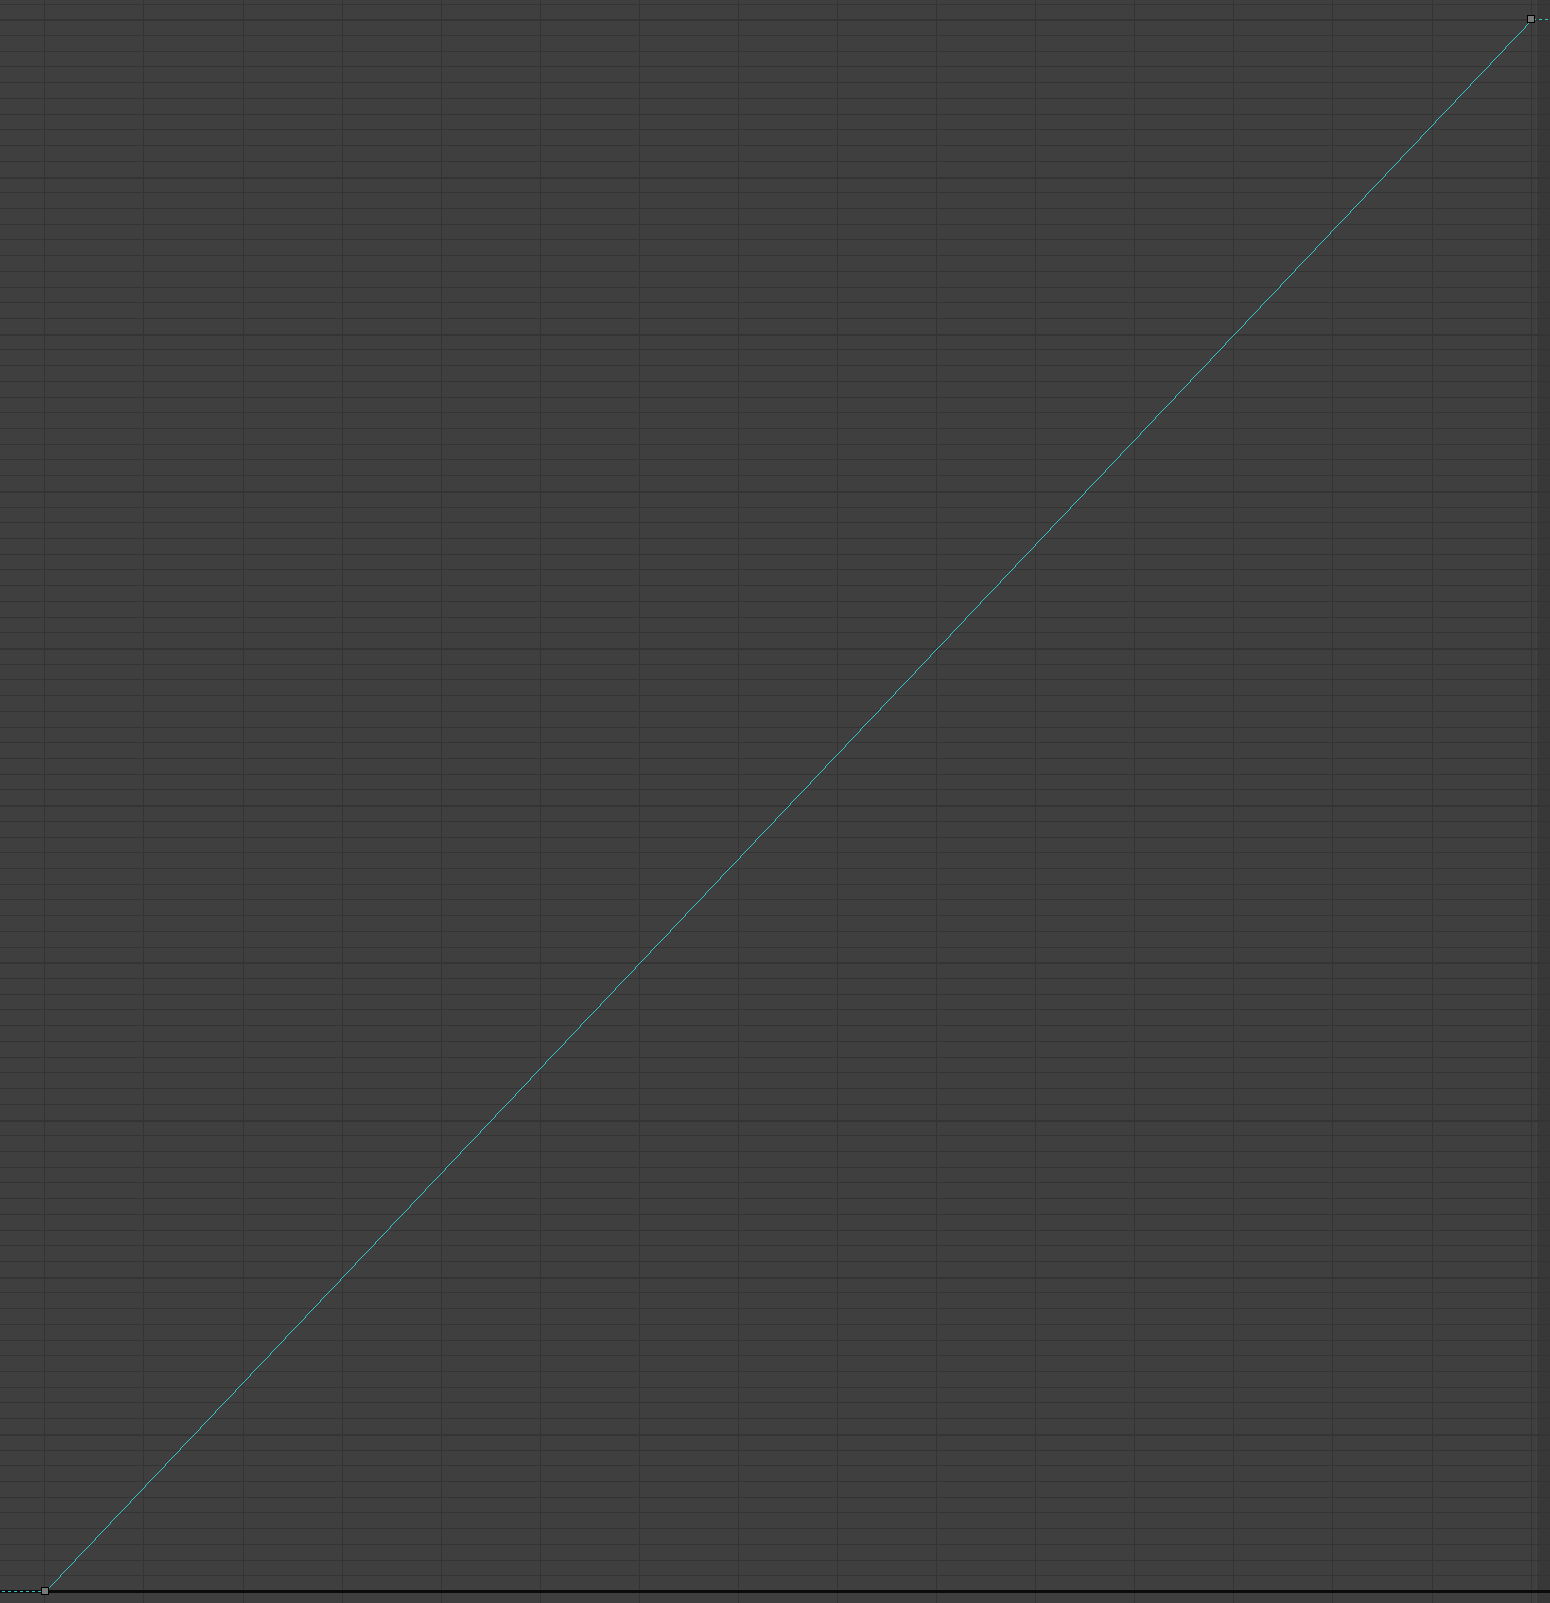
\includegraphics[width=0.5\textwidth]{imagenes/coche/pathConstraint.png}
   \caption{Curva del \textit{Path Constraint} que representa la posición del coche en el spline con respecto al tiempo.}
\end{figure}

Tras intentar de distintas formas modificar la forma de la curva del \textit{Path Constraint}, me ha sido imposible modificarla, por lo que la curva tiene forma lineal, que no es del todo realista, ya que un coche necesita un tiempo para acelerar y frenar.

\subsection{Movimiento de las ruedas}

Para hacer el movimiento de las ruedas, he usado \textit{Wire Parameter}, he seleccionado la rotación en el eje Y de una de ellas y la he unido a la caja del coche que tiene el \textit{Path Constraint}, más concretamente al porcentaje que ha recorrido en el spline. Esto lo he hecho así, ya que si hubiese elegido la posición en el eje X, al estar el coche en una zona que no fuera paralela a dicho eje, las ruedas girarían menos.

\bigskip

% QUIZAS COMPROBAR ESTO, QUE PUEDE SER QUE CAMBIE
En cuanto a la rotación, la he multiplicado por un factor de \rotFactor para que el giro realizado sea natural y más rápido de lo que tiene por defecto.

% foto del menu wire parameter
\begin{figure}[H]
    \centering
   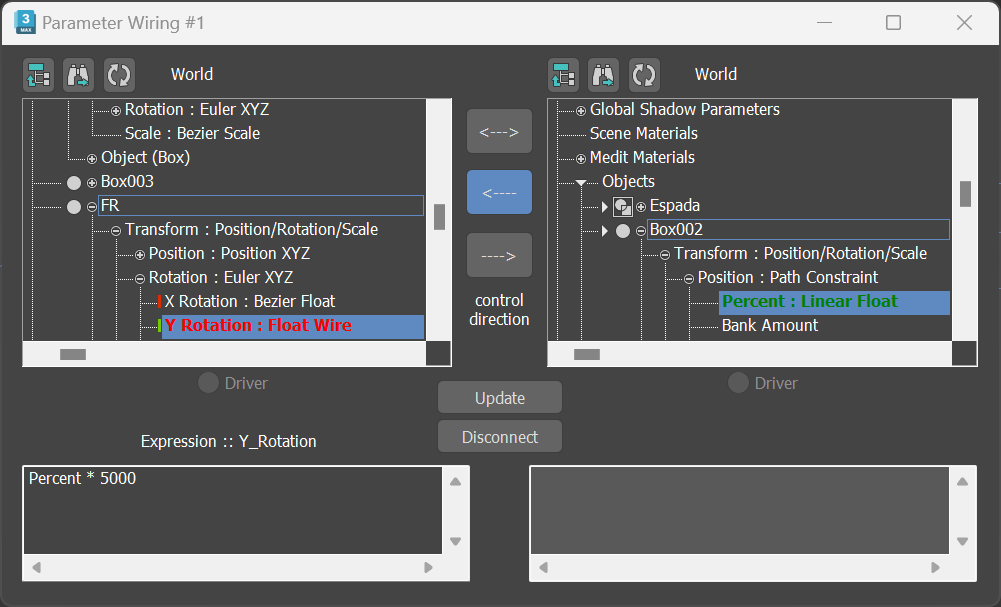
\includegraphics[width=0.6\textwidth]{imagenes/coche/wireFR.png}
   \caption{Menú con la configuración de la rueda.}
\end{figure}

Para simplificar futuros cambios en el factor de rotación, he asignado la rotación de las demás ruedas en el eje Y con la que tiene el porcentaje del spline, así se puede cambiar solo una vez el parámetro. Además, las ruedas del lado izquierdo deben tener un factor de -1 aplicado, ya que estas ruedas están rotadas 180 grados en el eje Z, haciendo que si no se usase girasen en el sentido contrario.

\begin{figure}[H]
    \centering
   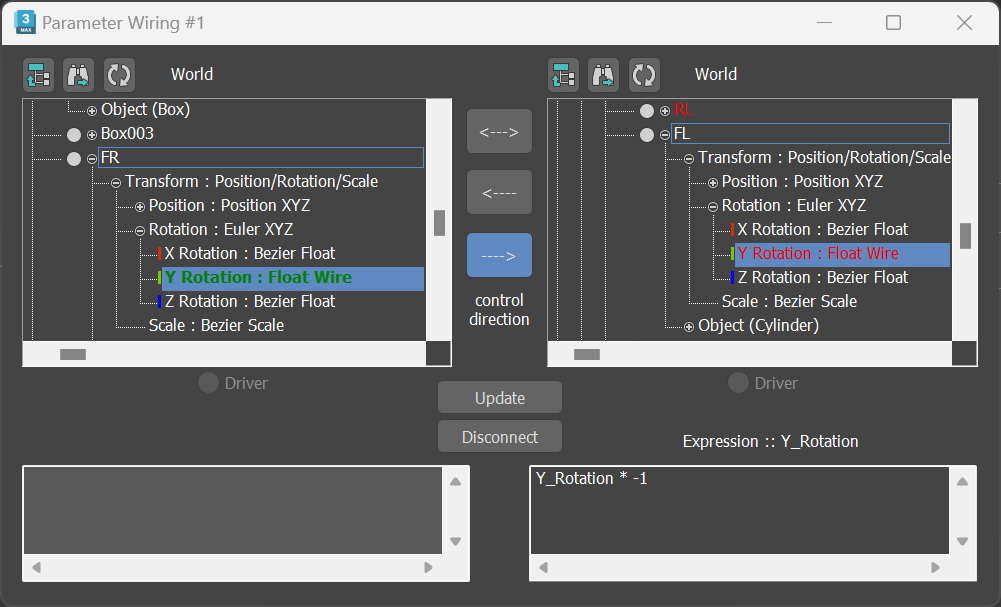
\includegraphics[width=0.6\textwidth]{imagenes/coche/wireFL.png}
   \caption{Ejemplo de la expresión utilizada para las ruedas de la izquierda.}
\end{figure}


Además, la configuración de la restricción es: 

\begin{figure}[H]
    \centering
   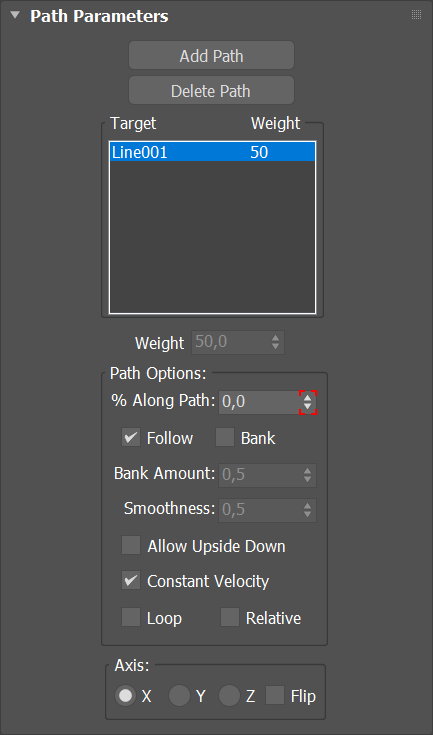
\includegraphics[width=0.3\textwidth]{imagenes/coche/config.png}
   \caption{Configuración del \textit{Path Constraint}.}
\end{figure}

\subsection{Resultado final}

Los fotogramas más importantes relativos al coche son:

% fotos
\begin{figure}[H]
    \centering
    \begin{subfigure}[t]{0.48\textwidth}
        \centering
        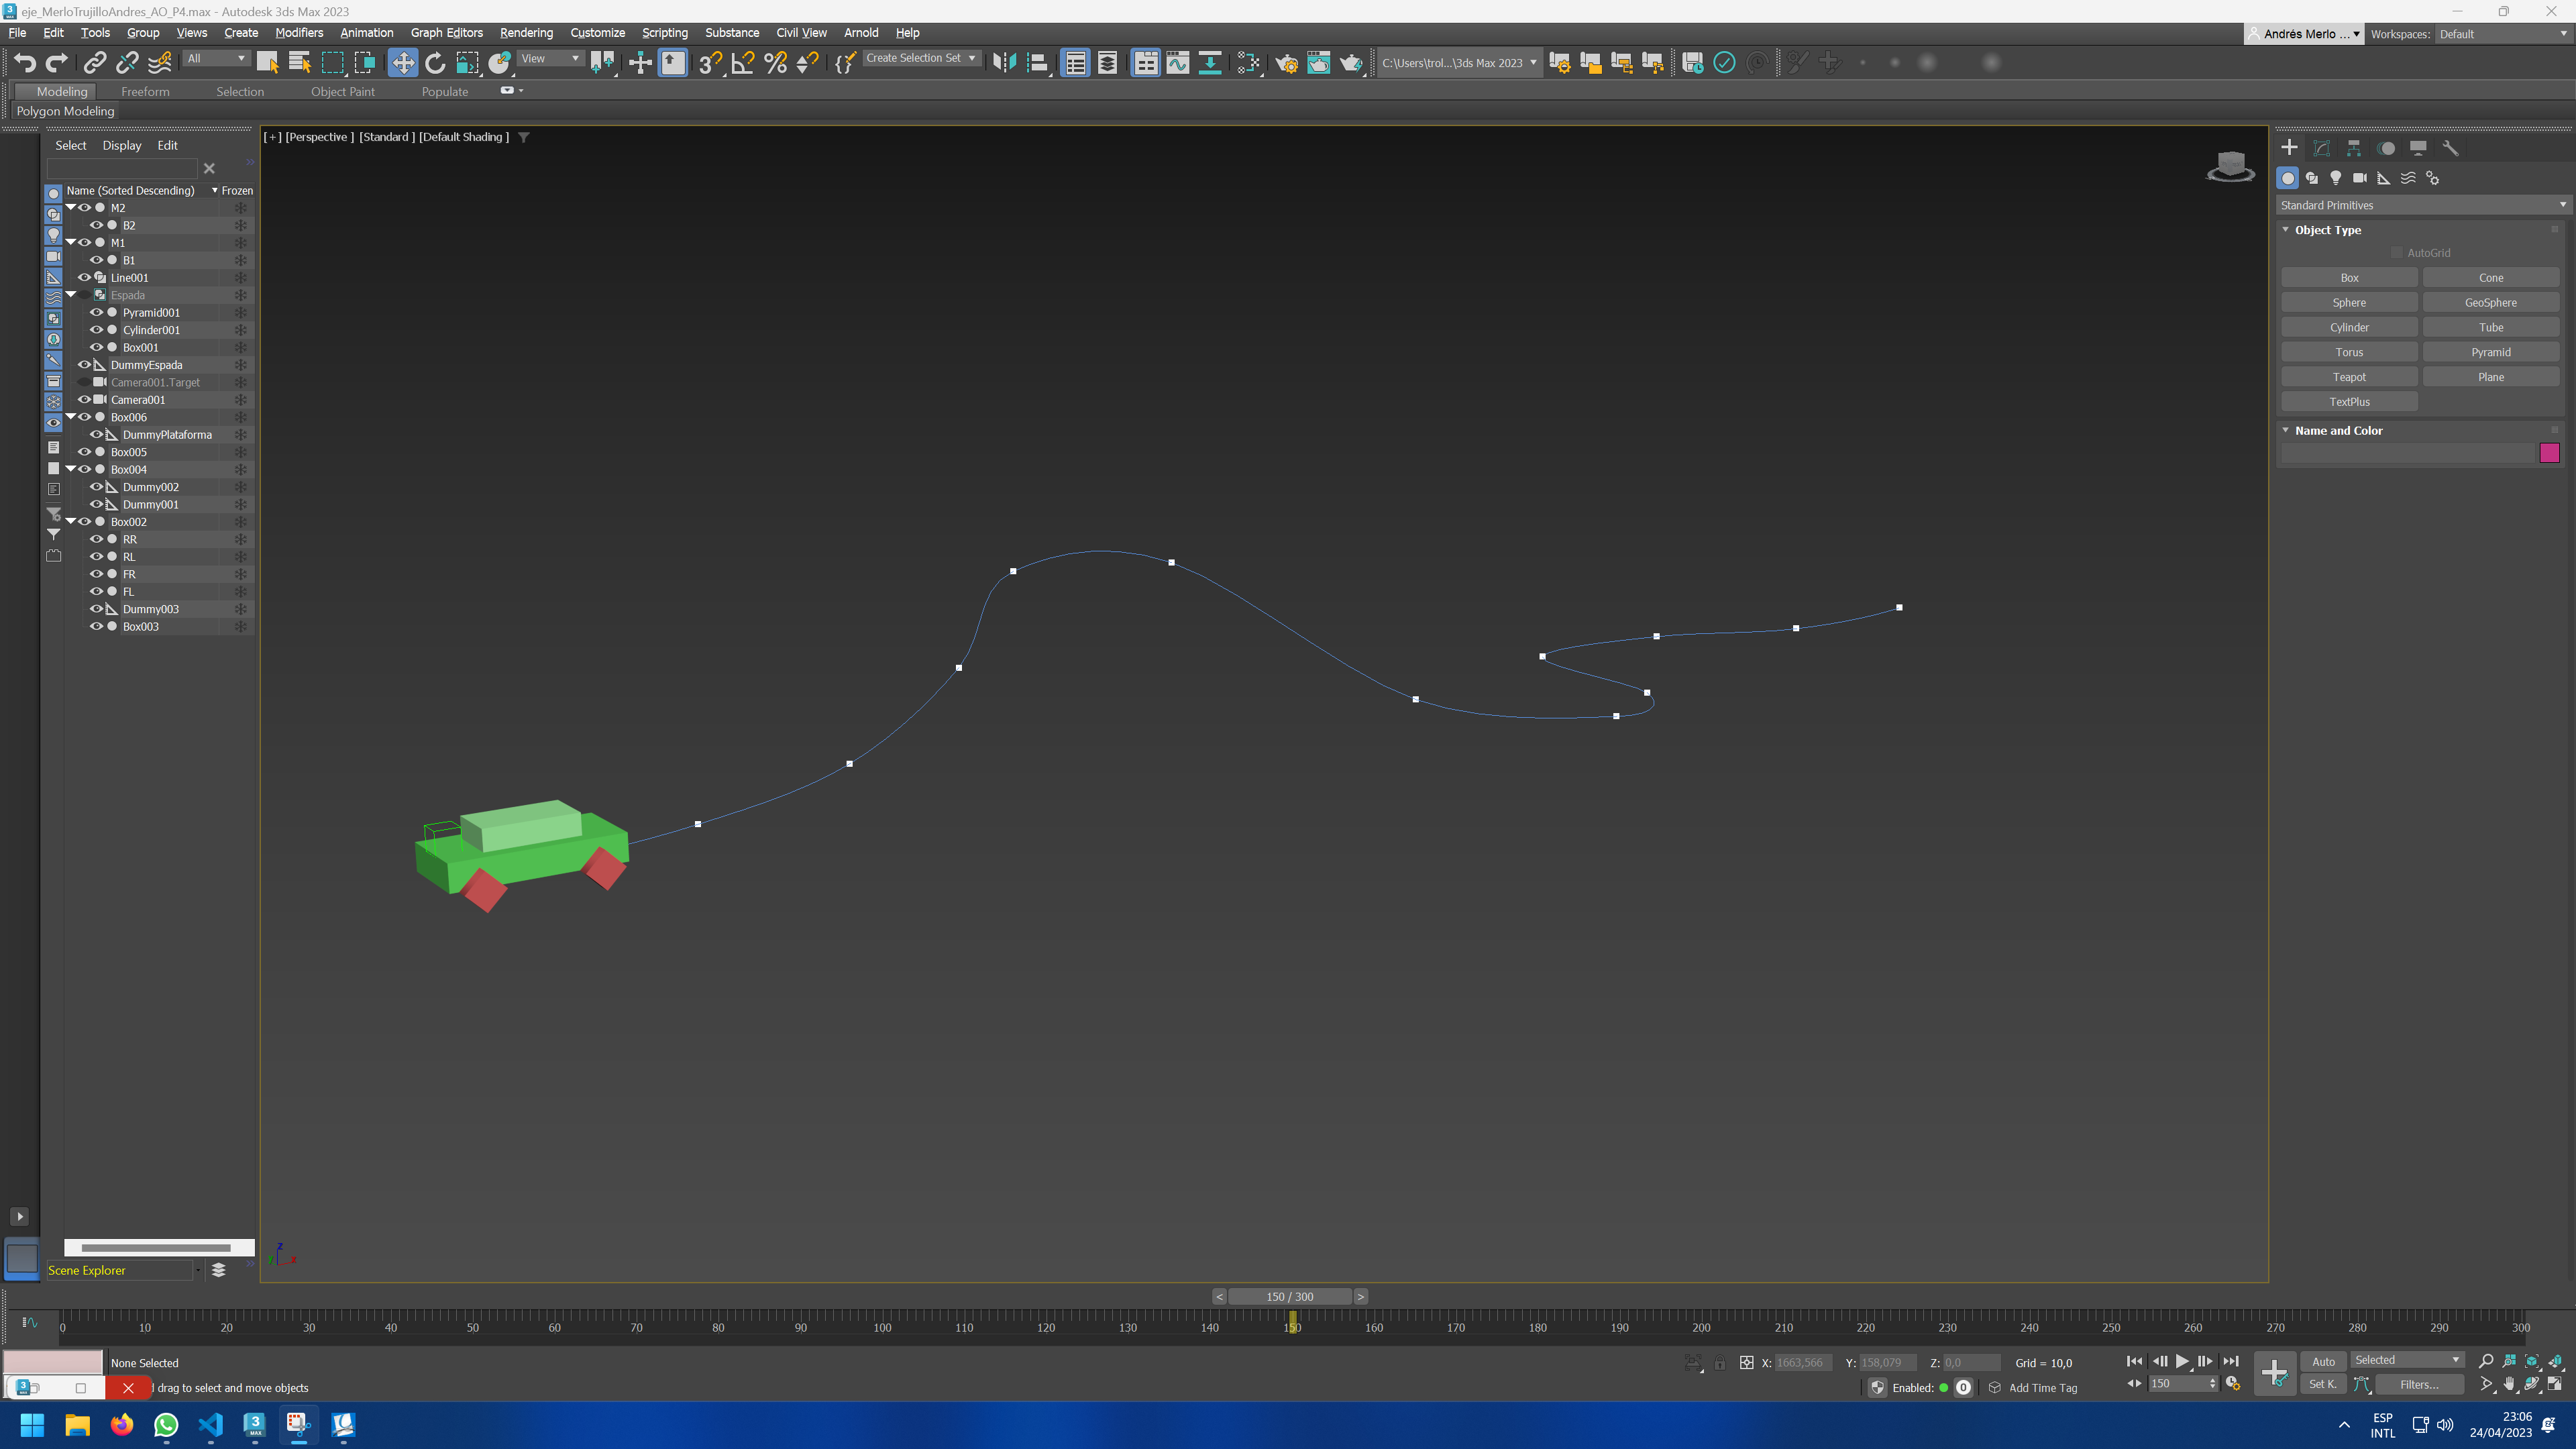
\includegraphics[width=\textwidth]{imagenes/coche/keyframes/150.png}
        \caption{Coche en el instante 150 y anteriores.}
    \end{subfigure}
    \hfill
    \begin{subfigure}[t]{0.48\textwidth}
        \centering
        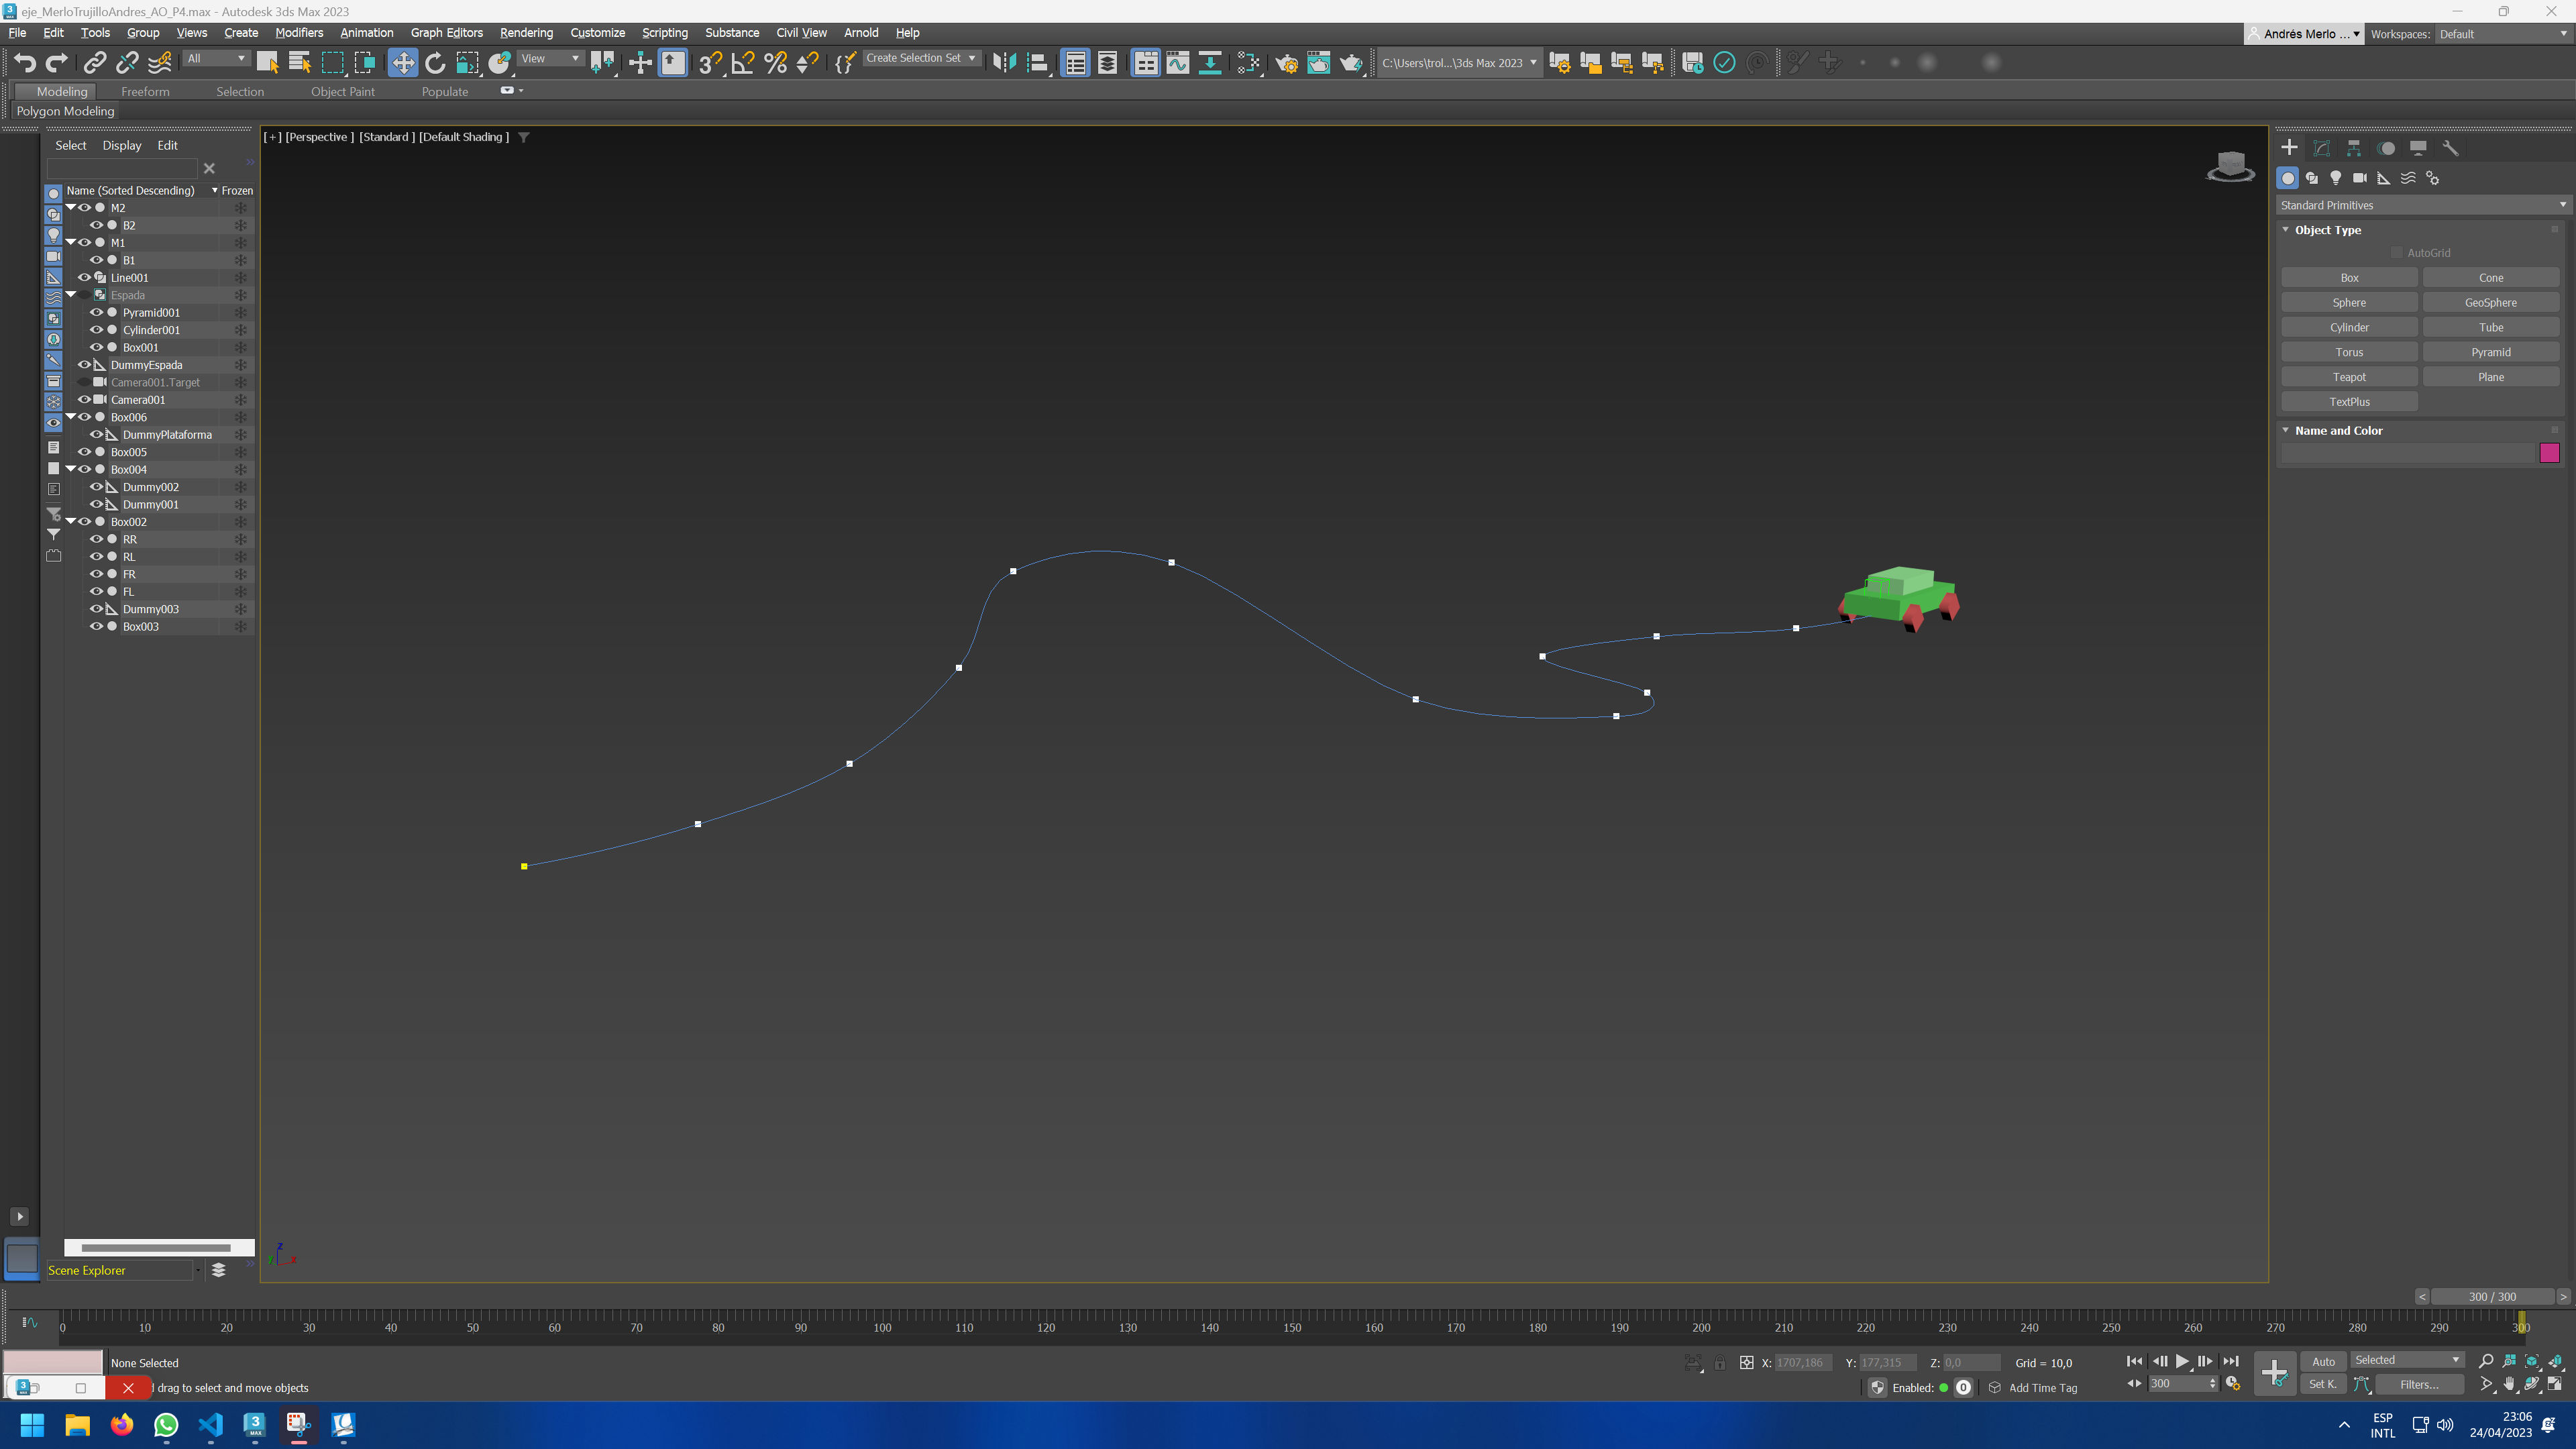
\includegraphics[width=\textwidth]{imagenes/coche/keyframes/300.png}
        \caption{Coche en el instante 300.}
    \end{subfigure}
    \caption{Instantes de la animación del \textit{Path Constraint}.}
\end{figure}

Y a continuación hay algunas capturas para mostrar la rotación de las ruedas:

\begin{figure}[H]
    \centering
    \begin{subfigure}[t]{0.48\textwidth}
        \centering
        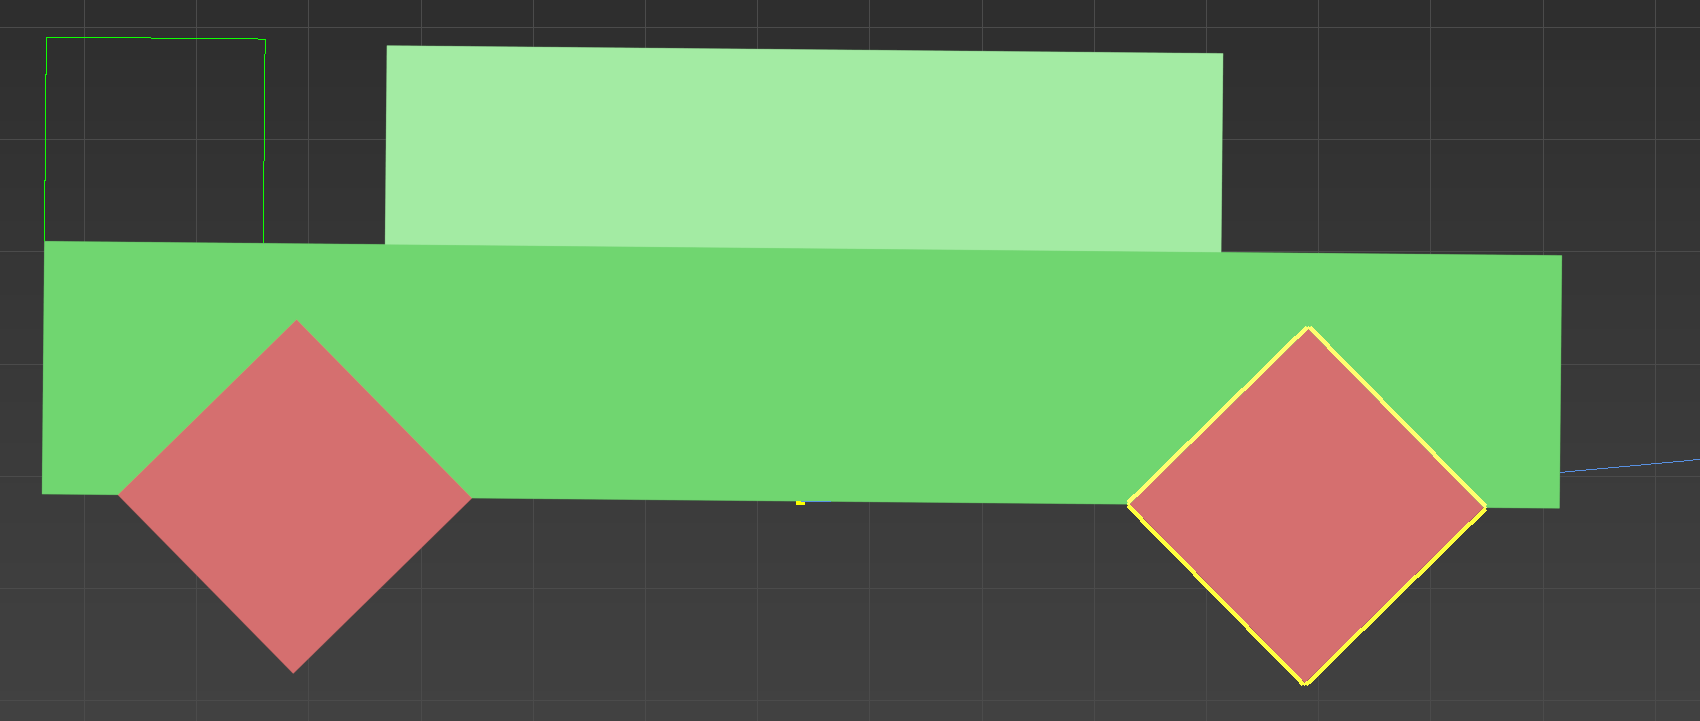
\includegraphics[width=\textwidth]{imagenes/coche/ruedas/antes.png}
        \caption{Ruedas de la derecha en el instante 150.}
    \end{subfigure}
    \hfill
    \begin{subfigure}[t]{0.48\textwidth}
        \centering
        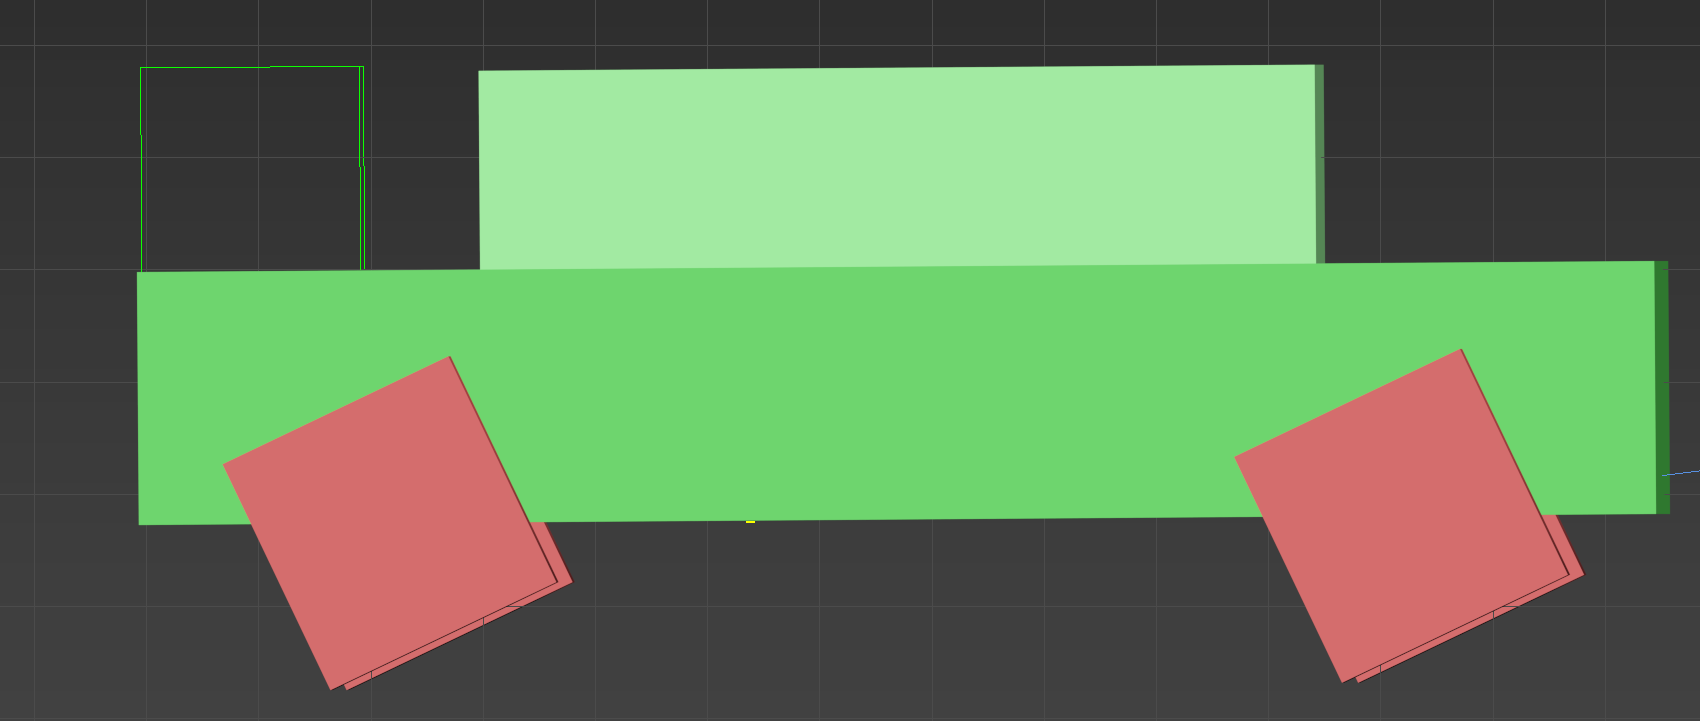
\includegraphics[width=\textwidth]{imagenes/coche/ruedas/despues.png}
        \caption{Rueda de la derecha en el instante 151.}
    \end{subfigure}
    \caption{Movimiento de las ruedas del coche.}
\end{figure}